\documentclass[aspectratio=169,11pt]{beamer}
\usepackage[T1]{fontenc}
\usepackage[utf8]{inputenc}
\usepackage[ngerman]{babel}
\usepackage{amsmath}
\usepackage{tikz}
\usepackage{qrcode}
\usetikzlibrary{arrows.meta,calc}
% An den bereitgestellten cgs-Beamerstil angelehnt; Inhalte bleiben deutsch.
\useinnertheme{rectangles}
\usepackage[libertine]{newtxmath}
\usepackage[default,light]{sourcesanspro}
\usepackage[default,bold]{sourcecodepro}
\usepackage[default,sfdefault,light,bold]{roboto}
\usepackage[final,babel]{microtype}
\usepackage{graphicx}

% Farben des Vorlagenstils; die Aliasnamen werden von den Foliengrafiken benutzt.
\definecolor{textblack}{cmyk}{0,0,0,1}
\definecolor{darkgray}{cmyk}{.10,0,0,.66}
\definecolor{lightgray}{cmyk}{.05,0,0,.33}
\definecolor{light}{cmyk}{0,0,0,.10}
\definecolor{hpi@gray}{RGB}{90,96,101}
\definecolor{hpi@red}{RGB}{177,6,58}
\definecolor{hpi@yellow}{RGB}{246,168,0}
\definecolor{hpi@orange}{RGB}{221,97,8}
\definecolor{hpi@blue}{RGB}{0,122,158}
\colorlet{ink}{textblack}
\colorlet{muted}{hpi@gray}
\colorlet{paper}{white}
\colorlet{soft}{light}
\colorlet{accent}{hpi@red}
\colorlet{blue}{hpi@blue}
\colorlet{sea}{hpi@blue}

\setbeamercolor{normal text}{fg=textblack,bg=white}
\setbeamercolor{background canvas}{bg=white}
\setbeamercolor{title}{fg=textblack}
\setbeamercolor{subtitle}{fg=textblack}
\setbeamercolor{author}{fg=textblack}
\setbeamercolor{institute}{fg=hpi@gray}
\setbeamercolor{frametitle}{fg=textblack,bg=white}
\setbeamercolor{footline}{fg=textblack,bg=white}
\setbeamercolor{structure}{fg=hpi@red}
\setbeamercolor{block title}{fg=textblack,bg=light}
\setbeamercolor{block body}{fg=textblack,bg=light}
\setbeamerfont{title}{size=\LARGE}
\setbeamerfont{subtitle}{size=\normalsize}
\setbeamerfont{author}{size=\normalsize}
\setbeamerfont{institute}{size=\small}
\setbeamerfont{frametitle}{size=\Large}
\setbeamerfont{footline}{size=\tiny}
\setbeamersize{text margin left=6mm,text margin right=6mm}
\setbeamertemplate{navigation symbols}{}
\setbeamertemplate{itemize items}[circle]
\setbeamercolor{itemize item}{fg=textblack}
\setbeamertemplate{itemize subitem}{$-$}
\setbeamercolor{itemize subitem}{fg=textblack}

% Ohne nachgelieferte Logos bleibt der Build nutzbar. Dateinamen wie in der Vorlage.
\newcommand{\logoplatz}[2]{%
  \IfFileExists{#1}{\includegraphics[width=14mm,height=5mm,keepaspectratio]{#1}}%
    {\fbox{\parbox[c][4mm][c]{12mm}{\centering\fontsize{4}{4}\selectfont #2}}}%
}
\newcommand{\cgslogos}{%
  \logoplatz{folien/logos/uni_logo.pdf}{Logo 1}\hspace{2mm}%
  \logoplatz{folien/logos/hpi-logo-cmyk.pdf}{Logo 2}%
}
\defbeamertemplate*{frametitle}{cgs-workshop}{%
  \begin{beamercolorbox}[ht=7mm,dp=1mm,wd=\paperwidth]{frametitle}%
    \hbox to \paperwidth{\hspace*{6mm}\usebeamerfont{frametitle}\insertframetitle\hfill\cgslogos\hspace*{6mm}}%
  \end{beamercolorbox}%
  \vspace{1mm}%
}
\defbeamertemplate*{footline}{cgs-workshop}{%
  \begin{beamercolorbox}[left,leftskip=6mm,rightskip=6mm,dp=3mm,wd=\paperwidth]{footline}%
    \usebeamerfont{footline}\insertframenumber%
    \ifx\insertsectionhead\empty\else\enspace|\enspace\insertsectionhead\fi%
    \hfill\insertshorttitle\quad\insertshortdate
  \end{beamercolorbox}%
}
\setbeamertemplate{frametitle}[cgs-workshop]
\setbeamertemplate{footline}[cgs-workshop]

\title[Grafiken programmieren]{Grafiken programmieren}
\subtitle{Mit Mathematik zu Millionen Pixeln}
\author{Willy Scheibel}
\institute{Marie-Curie-Gymnasium · Oberstufenworkshop}
\date{}
\setlength{\parskip}{3pt}
\newcommand{\tagline}[1]{{\color{accent}\footnotesize\bfseries\MakeUppercase{#1}}}
\newcommand{\frag}[1]{\texttt{#1}}
\newcommand{\qrplatz}[1]{\begin{tikzpicture}\node[draw=muted!60,rounded corners=2pt,minimum width=3.0cm,minimum height=1.1cm,align=center,text=muted,font=\scriptsize] {QR-Code: #1\\Adresse folgt};\end{tikzpicture}}
\newcommand{\demoheader}[1]{\tagline{Demo #1}\par\smallskip}
\newcommand{\hinweis}[1]{{\small\color{muted}#1}}
\newcommand{\bildrahmen}{\path[fill=soft,rounded corners=3pt] (0,0) rectangle (5.4,3.6);}
% Beide Folien verwenden dieselbe Skala: 0,275 cm pro Jahr ab 2000.
\newcommand{\zeitachse}{%
  \useasboundingbox (-6.2,-3.9) rectangle (7.6,.7);
  \draw[muted,thick] (0,0) -- (7.425,0);
  \foreach \jahr in {2000,2005,2010,2015,2020,2027} {
    \draw[muted] ({(\jahr-2000)*.275},0.07) -- +(0,-0.14);
    \node[font=\scriptsize,text=muted,above] at ({(\jahr-2000)*.275},.1) {\jahr};
  }
}
\newcommand{\zeitlabel}[2]{\node[overlay,anchor=east,align=right,font=\fontsize{7.3}{8}\selectfont,text=ink] at (-.25,#1) {#2};}
\newcommand{\zeitraum}[4]{%
  \zeitlabel{#1}{#2}
  \draw[sea,line width=3pt,line cap=round] ({(#3-2000)*.275},#1) -- ({(#4-2000)*.275},#1);
}
\newcommand{\zeitoffen}[3]{%
  \zeitlabel{#1}{#2}
  \draw[sea,line width=2pt,-{Stealth[length=2.5mm]}] ({(#3-2000)*.275},#1) -- (7.425,#1);
}
\newcommand{\zeitpunkt}[3]{%
  \zeitlabel{#1}{#2}
  \fill[accent] ({(#3-2000)*.275},#1) circle (2.3pt);
}

\begin{document}
\begin{frame}[plain]
\begin{beamercolorbox}[left,leftskip=0pt,ht=6mm,dp=1mm,wd=\textwidth]{frametitle}
  \hbox to \textwidth{\usebeamerfont{frametitle}\inserttitle\hfill\cgslogos}
\end{beamercolorbox}
\vspace{2mm}
\begin{center}
{\Large\bfseries ---\enspace\insertsubtitle\enspace---}\par\smallskip
\insertauthor\par\medskip
\begin{tikzpicture}[scale=.65]
\foreach \x in {0,...,6} \foreach \y in {0,...,6} {
  \pgfmathtruncatemacro{\tone}{15+8*\x+3*\y}
  \fill[sea!\tone!paper,rounded corners=1pt] (\x*.48,\y*.48) rectangle ++(.4,.4);
}
\fill[accent] (1.44,1.44) rectangle ++(.4,.4);
\end{tikzpicture}
\end{center}
\vfill\noindent{\footnotesize\color{muted}\insertinstitute}
\end{frame}

\section{Vorstellung}
\begin{frame}{Wer bin ich?}
\tagline{Willy Scheibel · Vom Hobby zum Studium}\par\vspace{3mm}
\begin{center}
\begin{tikzpicture}
\zeitachse
\zeitoffen{-.4}{ab 2003 · Hobbyprogrammierung}{2003}
\zeitoffen{-.94}{ab 2005 · Mitwirkung in Computerlehrgängen}{2005}
\zeitpunkt{-1.48}{2007 · Abitur}{2007}
\zeitraum{-2.02}{2007–2008 · Programmierjob und Zivildienst}{2007}{2008}
\zeitraum{-2.56}{2008–2010 · Werkstudent: Webseitenprogrammierung}{2008}{2010}
\zeitraum{-3.1}{2008–2011 · Bachelorstudium am HPI}{2008}{2011}
\zeitraum{-3.64}{2011–2014 · Masterstudium am HPI}{2011}{2014}
\end{tikzpicture}
\end{center}
\hinweis{Punkt: Ereignis · Balken: Zeitraum · Pfeil: Beginn bekannt, Ende offen}
\end{frame}

\begin{frame}{Was kam danach?}
\tagline{Willy Scheibel · Forschung, Praxis und Lehre}\par\vspace{3mm}
\begin{center}
\begin{tikzpicture}
\zeitachse
\zeitraum{-.4}{2011–2014 · Werkstudent: Computergrafik}{2011}{2014}
\zeitraum{-.94}{2011–2020 · Open Source in der Computergrafik}{2011}{2020}
\zeitoffen{-1.48}{ab 2014 · Promotionsstudium am HPI}{2014}
\zeitraum{-2.02}{2015–2022 · Miteigentümer einer Consulting-Firma\\Computergrafik}{2015}{2022}
\zeitoffen{-2.56}{ab 2015 · Internationale Publikationen\\Computergrafik und Visualisierung}{2015}
\zeitoffen{-3.1}{ab 2015 · Lehre\\Computergrafik und Software Engineering}{2015}
\zeitoffen{-3.64}{ab 2017 · Universitäre Selbstverwaltung}{2017}
\end{tikzpicture}
\end{center}
\hinweis{Pfeile markieren einen angegebenen Beginn; ein Ende ist nicht dargestellt.}
\end{frame}

\begin{frame}{Studium am HPI}
\tagline{Studium und Perspektiven}\vspace{2mm}
\begin{columns}[T,onlytextwidth]
\begin{column}{.56\textwidth}
{\small\bfseries Beispiel: Bachelor IT-Systems Engineering}\par\smallskip
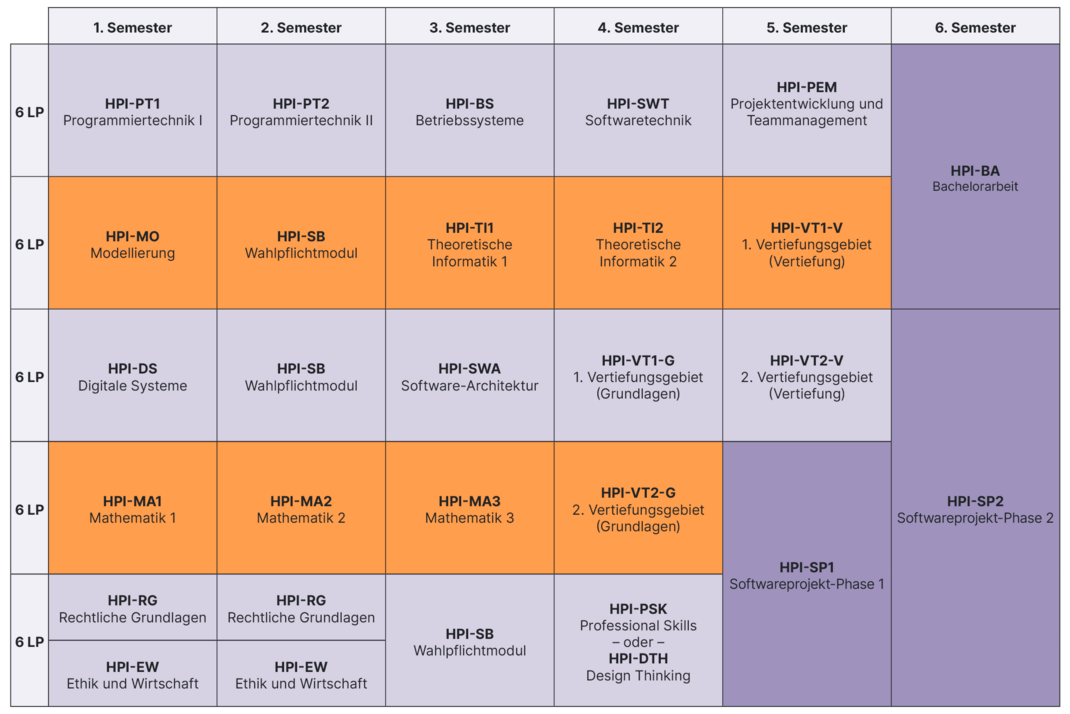
\includegraphics[width=\linewidth,height=4.1cm,keepaspectratio]{folien/bilder/hpi-studienverlaufsplan.png}\par
{\scriptsize\color{muted}Studienverlaufsplan · Quelle: \href{https://hpi.de}{Hasso-Plattner-Institut}}
\end{column}
\begin{column}{.40\textwidth}
{\small\bfseries Möglicher Studienweg}\par
{\small Bachelorstudium $\rightarrow$ Masterstudium $\rightarrow$ Promotion}\par\medskip
{\small\bfseries Mögliche Wege danach}\par
{\small Softwareentwicklung · Freelancing\\Gründung · Forschung}\par\medskip
\begin{columns}[c,onlytextwidth]
\begin{column}{1.5cm}
\href{https://hpi.de}{\colorbox{white}{\qrcode[height=1.15cm]{https://hpi.de}}}
\end{column}
\begin{column}{2.5cm}
\href{https://hpi.de}{\textcolor{sea}{\textbf{hpi.de}}}\par
{\scriptsize Infos zum Studium}
\end{column}
\end{columns}
\end{column}
\end{columns}
\end{frame}

\section{Einstieg}
\begin{frame}{Was machen wir heute?}
\tagline{Vom einzelnen Pixel zum Bild}\vspace{3mm}
\begin{center}
\begin{tikzpicture}[node distance=4mm, every node/.style={font=\small}]
\node[fill=soft,rounded corners,minimum width=2cm,minimum height=1cm] (a) at (0,0) {Farbe};
\node[fill=soft,rounded corners,minimum width=2cm,minimum height=1cm] (b) at (2.7,0) {Position};
\node[fill=soft,rounded corners,minimum width=2cm,minimum height=1cm] (c) at (5.4,0) {Formen};
\node[fill=soft,rounded corners,minimum width=2cm,minimum height=1cm] (d) at (8.1,0) {Bewegung};
\node[fill=soft,rounded corners,minimum width=2cm,minimum height=1cm] (e) at (10.8,0) {Noise};
\draw[-{Stealth},sea,thick] (a)--(b);\draw[-{Stealth},sea,thick] (b)--(c);\draw[-{Stealth},sea,thick] (c)--(d);\draw[-{Stealth},sea,thick] (d)--(e);
\end{tikzpicture}
\end{center}
\vspace{2mm}\begin{columns}[c]\begin{column}{.64\textwidth}Wir programmieren gemeinsam in ShaderToy.\\[2mm]Jedes Beispiel beginnt mit einem vorbereiteten Stand.\end{column}\begin{column}{.30\textwidth}\qrplatz{Website}\end{column}\end{columns}
\end{frame}

\begin{frame}{Ein Bild – viele Pixel}
\tagline{Einstieg · Tafelbild 1}\vspace{3mm}
\begin{columns}[c]
\begin{column}{.47\textwidth}
\begin{tikzpicture}[scale=.58]\fill[sea!35] (3,2) rectangle (4,3);\draw[step=1,muted!60] (0,0) grid (7,5);\draw[thick] (0,0) rectangle (7,5);\fill[accent] (3.5,2.5) circle (4pt);\draw[-{Stealth},accent,thick] (5.8,4.2)--(3.8,2.8);\node[anchor=west,font=\small] at (5.8,4.2) {dieses Pixel};\end{tikzpicture}
\end{column}
\begin{column}{.48\textwidth}
Für jedes Pixel berechnen wir eine Farbe.
\[\boxed{\text{Farbe}=f(x,y,t)}\]
\begin{itemize}\item Position im Bild\item Zeit seit dem Start\item Ergebnis: Rot, Grün und Blau\end{itemize}
\end{column}
\end{columns}
\end{frame}

\begin{frame}[fragile]{Die ShaderToy-Vorlage}
\tagline{Pro Pixel · Tafelbild 1}\vspace{2mm}
\begin{columns}[T]
\begin{column}{.55\textwidth}
\begin{block}{Ein minimales Image-Snippet}
\begin{verbatim}
void mainImage(out vec4 fragColor,
               in vec2 fragCoord)
{
    vec3 color = vec3(1.0);
    fragColor = vec4(color, 1.0);
}
\end{verbatim}
\end{block}
\end{column}
\begin{column}{.40\textwidth}
\begin{itemize}
\item \frag{fragCoord}: aktuelle Pixelposition
\item \frag{iResolution.xy}: Breite und Höhe
\item \frag{iTime}: Zeit in Sekunden
\item \frag{fragColor}: Ergebnisfarbe
\end{itemize}
\hinweis{Die Vorlage ist ein vollständiges ShaderToy-Snippet.}
\end{column}
\end{columns}
\end{frame}

\section{Demos}
\begin{frame}{Wie entsteht eine Farbe?}
\demoheader{1 · Farbe und Zeit}
\begin{columns}[c]
\begin{column}{.48\textwidth}
\begin{itemize}\item Ein RGB-Vektor färbt alle Pixel gleich.\item Was passiert, wenn sich die Werte ändern?\item \frag{iTime} lässt die Farbe schwingen.\end{itemize}
\medskip\qrplatz{ShaderToy-START}
\end{column}
\begin{column}{.48\textwidth}
\begin{tikzpicture}\bildrahmen
\foreach \i/\name/\col/\val in {0/Rot/accent/3.8,1/Grün/sea/2.8,2/Blau/blue/4.3}{\node[anchor=east,font=\small] at (1.2,2.8-\i*.85) {\name};\fill[white] (1.4,2.65-\i*.85) rectangle (4.9,2.95-\i*.85);\fill[\col] (1.4,2.65-\i*.85) rectangle (\val,2.95-\i*.85);}
\end{tikzpicture}\par\hinweis{Tafelbild 2 · Werte zwischen 0 und 1}
\end{column}
\end{columns}
\end{frame}

\begin{frame}{Was verrät die Position?}
\demoheader{2 · Pixelposition und Farbverlauf}
\begin{columns}[c]
\begin{column}{.48\textwidth}
\begin{itemize}\item Pixelposition durch die Bildgröße teilen.\item Position als Farbanteil sichtbar machen.\item Zwei Farben entlang der x-Achse mischen.\end{itemize}
\qrplatz{ShaderToy-START}
\end{column}
\begin{column}{.48\textwidth}
\begin{tikzpicture}\bildrahmen
\shade[left color=blue,right color=accent] (.5,.6) rectangle (4.9,3);
\draw[-{Stealth},white,very thick] (.8,1)--(4.6,1);
\node[white,font=\small,above] at (1.1,1) {links};\node[white,font=\small,above] at (4.2,1) {rechts};
\end{tikzpicture}\par\hinweis{Tafelbild 3 · Position und Auflösung}
\end{column}
\end{columns}
\end{frame}

\begin{frame}{Wie werden aus Abständen Formen?}
\demoheader{3 · Kreis und bewegte Metaballs}
\begin{columns}[c]
\begin{column}{.48\textwidth}
\begin{itemize}\item Abstand zum Mittelpunkt entscheidet über die Farbe.\item Felder mehrerer Zentren addieren.\item Mit \frag{iTime} bewegen sich die Zentren.\end{itemize}
\qrplatz{ShaderToy-START}
\end{column}
\begin{column}{.48\textwidth}
\begin{tikzpicture}\bildrahmen
\fill[sea!85] (2,1.8) circle (1.0);\fill[sea!85] (3.4,1.8) circle (1.0);\fill[sea!85] (2.7,1.8) ellipse (.6 and .7);
\fill[white] (2,1.8) circle (2pt) (3.4,1.8) circle (2pt);
\draw[white,-{Stealth},thick] (1.9,.65)--(1.2,.65);\draw[white,-{Stealth},thick] (3.5,.65)--(4.2,.65);
\end{tikzpicture}\par\hinweis{Tafelbilder 4–5 · Abstand und Felder}
\end{column}
\end{columns}
\end{frame}

\begin{frame}{Was macht eine Kante weich?}
\demoheader{4 · Polynom und weiche Kante}
\begin{columns}[c]
\begin{column}{.48\textwidth}
\begin{itemize}\item Harte Grenze durch einen Übergang ersetzen.\item Farben zunächst linear mischen.\item Ein Polynom glättet beide Enden.\end{itemize}
\qrplatz{ShaderToy-START}
\end{column}
\begin{column}{.48\textwidth}
\begin{tikzpicture}\bildrahmen
\draw[-{Stealth},muted] (.6,.6)--(4.8,.6) node[right] {\scriptsize $t$};
\draw[-{Stealth},muted] (.6,.6)--(.6,3.1);
\draw[dashed,muted] (.6,.6)--(4.5,2.8);
\draw[sea,very thick,domain=0:1,samples=50] plot ({.6+3.9*\x},{.6+2.2*(3*\x*\x-2*\x*\x*\x)});
\node[font=\small,text=sea] at (2.8,1.15) {$3t^2-2t^3$};
\end{tikzpicture}\par\hinweis{Tafelbild 6 · Randbedingungen}
\end{column}
\end{columns}
\end{frame}

\begin{frame}{Wie bewegt sich eine Welle?}
\demoheader{5 · Sinus und Animation}
\begin{columns}[c]
\begin{column}{.48\textwidth}
\begin{itemize}\item Der Sinus ordnet jeder x-Position eine Höhe zu.\item Amplitude und Frequenz verändern die Form.\item Die Zeit verschiebt die Phase.\end{itemize}
\qrplatz{ShaderToy-START}
\end{column}
\begin{column}{.48\textwidth}
\begin{tikzpicture}\bildrahmen
\draw[-{Stealth},muted] (.4,1.8)--(5,1.8);\draw[-{Stealth},muted] (.8,.3)--(.8,3.25);
\draw[sea,very thick,domain=0:4.1,samples=80] plot ({.8+\x},{1.8+.9*sin(\x*135)});
\draw[accent,dashed,thick,domain=0:4.1,samples=80] plot ({.8+\x},{1.8+.9*sin(\x*135-55)});
\end{tikzpicture}\par\hinweis{Tafelbild 7 · Das spätere Bildmotiv ist noch offen.}
\end{column}
\end{columns}
\end{frame}

\begin{frame}{Wie genau ist eine Näherung?}
\demoheader{6 · Taylorapproximation}
\begin{columns}[c]
\begin{column}{.48\textwidth}
\begin{itemize}\item Sinus und ein Polynom vergleichen.\item Nahe $x=0$ liegen die Kurven zusammen.\item Weiter entfernt wird der Unterschied sichtbar.\end{itemize}
\qrplatz{ShaderToy-START}
\end{column}
\begin{column}{.48\textwidth}
\begin{tikzpicture}\bildrahmen
\draw[-{Stealth},muted] (.3,1.8)--(5,1.8);\draw[-{Stealth},muted] (2.7,.3)--(2.7,3.2);
\draw[sea,very thick,domain=-3.2:3.2,samples=80] plot ({2.7+.67*\x},{1.8+sin(\x r)});
\draw[accent,dashed,thick,domain=-3.2:3.2,samples=80] plot ({2.7+.67*\x},{1.8+\x-\x*\x*\x/6+\x*\x*\x*\x*\x/120});
\node[font=\small] at (2.7,.45) {$x-\frac{x^3}{6}+\frac{x^5}{120}$};
\end{tikzpicture}\par\hinweis{Tafelbild 8 · Näherung um $x=0$}
\end{column}
\end{columns}
\end{frame}

\begin{frame}{Wie wird Zufall zu einem Muster?}
\demoheader{7 · Value Noise}
\begin{columns}[c]
\begin{column}{.48\textwidth}
\begin{itemize}\item Pseudozufallswerte an Gitterpunkten.\item Zwischen benachbarten Werten mischen.\item Das bekannte Polynom glättet Übergänge.\end{itemize}
\qrplatz{ShaderToy-START}
\end{column}
\begin{column}{.48\textwidth}
\begin{tikzpicture}\bildrahmen
\fill[sea!20] (2,1) rectangle (3,2);\draw[step=1,muted] (1,.5) grid (4,3.5);
\foreach \x in {1,2,3,4} \foreach \y in {1,2,3} \fill[sea] (\x,\y) circle (2.6pt);
\fill[accent] (2.5,1.45) circle (3pt);\node[font=\small,anchor=west] at (2.6,1.45) {Pixel};
\end{tikzpicture}\par\hinweis{Tafelbild 9 · Gitter und Interpolation}
\end{column}
\end{columns}
\end{frame}

\begin{frame}{Wie entstehen feine Wolkenstrukturen?}
\demoheader{8 · fBm}
\begin{columns}[c]
\begin{column}{.48\textwidth}
\begin{itemize}\item Noise in verschiedenen Größen verwenden.\item Große und kleine Strukturen gewichten.\item Mehrere Oktaven überlagern.\end{itemize}
\qrplatz{ShaderToy-START}
\end{column}
\begin{column}{.48\textwidth}
\begin{tikzpicture}\bildrahmen
\draw[sea,step=.6] (.4,1) grid (1.6,2.2);\draw[sea,step=.3] (2.1,1) grid (3.3,2.2);\draw[sea,step=.15] (3.8,1) grid (5,2.2);
\node at (1.85,1.6) {$+$};\node at (3.55,1.6) {$+$};
\node[font=\small] at (2.7,.5) {grob \qquad\quad fein};
\end{tikzpicture}\par\hinweis{Tafelbild 10 · Frequenz und Gewicht}
\end{column}
\end{columns}
\end{frame}

\section{Ausblick}
\begin{frame}{Was ist noch möglich?}
\tagline{Inspirationsgalerie · Beispiele folgen}\vspace{4mm}
\begin{columns}[T]
\begin{column}{.31\textwidth}\begin{block}{Rotation}Matrizen verändern Koordinaten.\end{block}\end{column}
\begin{column}{.31\textwidth}\begin{block}{Ray Marching}Abstände helfen, räumliche Szenen zu erkunden.\end{block}\end{column}
\begin{column}{.31\textwidth}\begin{block}{Stochastik}Zufällige Verfahren erzeugen komplexe Effekte.\end{block}\end{column}
\end{columns}
\vspace{3mm}\hinweis{Konkrete Beispiele und Quellen werden noch ausgewählt.}
\end{frame}

\begin{frame}{Was nehmen wir mit?}
\tagline{Rückblick und Fragen}\vspace{3mm}
\begin{columns}[c]
\begin{column}{.62\textwidth}
\begin{itemize}\item Ein Shader berechnet eine Farbe pro Pixel.\item Position und Zeit machen Bilder veränderlich.\item Mathematik verbindet einfache Regeln zu Mustern.\end{itemize}
\medskip{\large\bfseries Was würdet ihr als Nächstes verändern?}
\end{column}
\begin{column}{.32\textwidth}\qrplatz{Website}\par\medskip\hinweis{Demos und Materialien · Adresse folgt}\end{column}
\end{columns}
\end{frame}
\end{document}
